%\RequirePackage{pdfmanagement-testphase}
%\RequirePackage{latex-lab}
%\RequirePackage{tagpdf}
\DocumentMetadata{%
 %  uncompress, %only for debugging!!
  pdfversion=2.0,
  testphase={phase-II, tabular, graphic}%
  % testphase={phase-II,math, tabular, graphic}% TOC Does not work
  % testphase={phase-III,math}% TOC works
}
\tagpdfsetup{activate, tabsorder=structure}
% Use the following to fix bug in November 2023 download of LaTeX
\ExplSyntaxOn
\cs_generate_variant:Nn\__tag_prop_gput:Nnn{cnx}
\ExplSyntaxOff
%

% Options for packages loaded elsewhere
\PassOptionsToPackage{unicode}{hyperref}
\PassOptionsToPackage{hyphens}{url}
\PassOptionsToPackage{dvipsnames,svgnames,x11names}{xcolor}
%
\documentclass[
]{scrartcl}

\usepackage{amsmath,amssymb}
\usepackage{iftex}
\ifPDFTeX
  \usepackage[T1]{fontenc}
  \usepackage[utf8]{inputenc}
  \usepackage{textcomp} % provide euro and other symbols
\else % if luatex or xetex
  \usepackage{unicode-math}
  \defaultfontfeatures{Scale=MatchLowercase}
  \defaultfontfeatures[\rmfamily]{Ligatures=TeX,Scale=1}
\fi
\usepackage{lmodern}
\ifPDFTeX\else
    % xetex/luatex font selection
\fi
% Use upquote if available, for straight quotes in verbatim environments
\IfFileExists{upquote.sty}{\usepackage{upquote}}{}
\IfFileExists{microtype.sty}{% use microtype if available
  \usepackage[]{microtype}
  \UseMicrotypeSet[protrusion]{basicmath} % disable protrusion for tt fonts
}{}
\makeatletter
\@ifundefined{KOMAClassName}{% if non-KOMA class
  \IfFileExists{parskip.sty}{%
    \usepackage{parskip}
  }{% else
    \setlength{\parindent}{0pt}
    \setlength{\parskip}{6pt plus 2pt minus 1pt}}
}{% if KOMA class
  \KOMAoptions{parskip=half}}
\makeatother
\usepackage{xcolor}
\setlength{\emergencystretch}{3em} % prevent overfull lines
\setcounter{secnumdepth}{5}
% Make \paragraph and \subparagraph free-standing
\ifx\paragraph\undefined\else
  \let\oldparagraph\paragraph
  \renewcommand{\paragraph}[1]{\oldparagraph{#1}\mbox{}}
\fi
\ifx\subparagraph\undefined\else
  \let\oldsubparagraph\subparagraph
  \renewcommand{\subparagraph}[1]{\oldsubparagraph{#1}\mbox{}}
\fi


\providecommand{\tightlist}{%
  \setlength{\itemsep}{0pt}\setlength{\parskip}{0pt}}\usepackage{longtable,booktabs,array}
\usepackage{calc} % for calculating minipage widths
% Correct order of tables after \paragraph or \subparagraph
\usepackage{etoolbox}
\makeatletter
\patchcmd\longtable{\par}{\if@noskipsec\mbox{}\fi\par}{}{}
\makeatother
% Allow footnotes in longtable head/foot
\IfFileExists{footnotehyper.sty}{\usepackage{footnotehyper}}{\usepackage{footnote}}
\makesavenoteenv{longtable}
\usepackage{graphicx}
\makeatletter
\def\maxwidth{\ifdim\Gin@nat@width>\linewidth\linewidth\else\Gin@nat@width\fi}
\def\maxheight{\ifdim\Gin@nat@height>\textheight\textheight\else\Gin@nat@height\fi}
\makeatother
% Scale images if necessary, so that they will not overflow the page
% margins by default, and it is still possible to overwrite the defaults
% using explicit options in \includegraphics[width, height, ...]{}
\setkeys{Gin}{width=\maxwidth,height=\maxheight,keepaspectratio}
% Set default figure placement to htbp
\makeatletter
\def\fps@figure{htbp}
\makeatother
% definitions for citeproc citations
\NewDocumentCommand\citeproctext{}{}
\NewDocumentCommand\citeproc{mm}{%
  \begingroup\def\citeproctext{#2}\cite{#1}\endgroup}
\makeatletter
 % allow citations to break across lines
 \let\@cite@ofmt\@firstofone
 % avoid brackets around text for \cite:
 \def\@biblabel#1{}
 \def\@cite#1#2{{#1\if@tempswa , #2\fi}}
\makeatother
\newlength{\cslhangindent}
\setlength{\cslhangindent}{1.5em}
\newlength{\csllabelwidth}
\setlength{\csllabelwidth}{3em}
\newenvironment{CSLReferences}[2] % #1 hanging-indent, #2 entry-spacing
 {\begin{list}{}{%
  \setlength{\itemindent}{0pt}
  \setlength{\leftmargin}{0pt}
  \setlength{\parsep}{0pt}
  % turn on hanging indent if param 1 is 1
  \ifodd #1
   \setlength{\leftmargin}{\cslhangindent}
   \setlength{\itemindent}{-1\cslhangindent}
  \fi
  % set entry spacing
  \setlength{\itemsep}{#2\baselineskip}}}
 {\end{list}}
\usepackage{calc}
\newcommand{\CSLBlock}[1]{\hfill\break\parbox[t]{\linewidth}{\strut\ignorespaces#1\strut}}
\newcommand{\CSLLeftMargin}[1]{\parbox[t]{\csllabelwidth}{\strut#1\strut}}
\newcommand{\CSLRightInline}[1]{\parbox[t]{\linewidth - \csllabelwidth}{\strut#1\strut}}
\newcommand{\CSLIndent}[1]{\hspace{\cslhangindent}#1}

\usepackage{hyphenat}
\usepackage{graphicx}
% and their extensions so you won't have to specify these with
 % every instance of \includegraphics
\usepackage{pdfcomment}
\DeclareGraphicsExtensions{.pdf,.jpeg,.png}
\usepackage{wallpaper} % for the background image on title page
\usepackage{geometry}
% set font
\usepackage{fontspec}
\setsansfont[Ligatures=TeX]{Arial Narrow}
\usepackage[headsepline=0.005pt:,footsepline=0.005pt:,plainfootsepline,automark]{scrlayer-scrpage}
\clearpairofpagestyles
\ohead[]{\headmark} \cofoot[\pagemark]{\pagemark}
\lohead{Petrale sole assessment 2023}
\ModifyLayer[addvoffset=-.6ex]{scrheadings.foot.above.line}
\ModifyLayer[addvoffset=-.6ex]{plain.scrheadings.foot.above.line}
\setkomafont{pageheadfoot}{\small}

\makeatletter
\@ifpackageloaded{caption}{}{\usepackage{caption}}
\AtBeginDocument{%
\ifdefined\contentsname
  \renewcommand*\contentsname{Table of contents}
\else
  \newcommand\contentsname{Table of contents}
\fi
\ifdefined\listfigurename
  \renewcommand*\listfigurename{List of Figures}
\else
  \newcommand\listfigurename{List of Figures}
\fi
\ifdefined\listtablename
  \renewcommand*\listtablename{List of Tables}
\else
  \newcommand\listtablename{List of Tables}
\fi
\ifdefined\figurename
  \renewcommand*\figurename{Figure}
\else
  \newcommand\figurename{Figure}
\fi
\ifdefined\tablename
  \renewcommand*\tablename{Table}
\else
  \newcommand\tablename{Table}
\fi
}
\@ifpackageloaded{float}{}{\usepackage{float}}
\floatstyle{ruled}
\@ifundefined{c@chapter}{\newfloat{codelisting}{h}{lop}}{\newfloat{codelisting}{h}{lop}[chapter]}
\floatname{codelisting}{Listing}
\newcommand*\listoflistings{\listof{codelisting}{List of Listings}}
\makeatother
\makeatletter
\makeatother
\makeatletter
\@ifpackageloaded{caption}{}{\usepackage{caption}}
\@ifpackageloaded{subcaption}{}{\usepackage{subcaption}}
\makeatother
\ifLuaTeX
\usepackage[bidi=basic]{babel}
\else
\usepackage[bidi=default]{babel}
\fi
\babelprovide[main,import]{english}
% get rid of language-specific shorthands (see #6817):
\let\LanguageShortHands\languageshorthands
\def\languageshorthands#1{}
\ifLuaTeX
  \usepackage{selnolig}  % disable illegal ligatures
\fi
\usepackage{bookmark}

\IfFileExists{xurl.sty}{\usepackage{xurl}}{} % add URL line breaks if available
\urlstyle{same} % disable monospaced font for URLs
\hypersetup{
  pdftitle={Status of the Petrale sole stock in U.S. waters off the coast of U.S. West Coast in 2023},
  pdfauthor={Ian G. Taylor; Vladlena Gertseva; Nick Tolimieri},
  pdflang={en},
  colorlinks=true,
  linkcolor={blue},
  filecolor={Maroon},
  citecolor={Blue},
  urlcolor={Blue},
  pdfcreator={LaTeX via pandoc}}

\title{Status of the Petrale sole stock in U.S. waters off the coast of
U.S. West Coast in 2023}
\author{Ian G. Taylor \and Vladlena Gertseva \and Nick Tolimieri}
\date{2024-10-30}

\begin{document}
  \begin{titlepage}
  % This is a combination of Pandoc templating and LaTeX
  % Pandoc templating https://pandoc.org/MANUAL.html#templates
  % See the README for help

  \newgeometry{top=2in,bottom=1in,right=1in,left=1in}
  \begin{minipage}[b][\textheight][s]{\textwidth}
  \raggedright

  % \includegraphics[width=2cm]{NOAA_Transparent_Logo.png}

  % background image


  % Title and subtitle
  {\huge\bfseries\nohyphens{Status of the Petrale sole stock in U.S.
  waters off the coast of U.S. West Coast in 2023}}\\[1\baselineskip]


  \vspace{1\baselineskip}

  %%%%%% Cover image
  \pdftooltip{\includegraphics{support\_files/Petrale\_sole.png}}{An illustration of petrale sole}
  %\includegraphics[alt={An illustration of petrale sole},width=10cm]{support\_files/Petrale\_sole.png}

  \vspace{1\baselineskip}

  % Authors
  % This hairy bit of code is just to get "and" between the last 2
  % authors. See below if you don't need that
   {\large{Ian G. Taylor}}{\textsuperscript{1}}%
  %
  ,
   {\large{Vladlena Gertseva}}{\textsuperscript{1}}%
  %
  %
  { and \large{Nick Tolimieri}}%
  {\textsuperscript{1}}%
  %


  % This is how to do it if you don't need the "and"

  %%%%%% Affiliations
  \vspace{2\baselineskip}

  \hangindent=1em
  \hangafter=1
  %
  {1}.~{NOAA Fisheries Northwest Fisheries Science Center}%
  %
  %
  , %
  {2725 Montlake Boulevard East}%
  %


  %%%%%% Correspondence
  \vspace{1\baselineskip}


  %use \vfill instead to get the space to fill flexibly
  %\vspace{0.25\textheight} % Whitespace between the title block and the publisher

  \vfill


  % Whitespace between the title block and the tagline
  \vspace{1\baselineskip}

  %%%%%% Tagline at bottom
  
\includegraphics[width=2cm]{support_files/us_doc_logo.png}\newline
  U.S. Department of Commerce\newline
  National Oceanic and Atmospheric Administration\newline
  National Marine Fisheries Service\newline
  Northwest Fisheries Science Center\newline

  \end{minipage}
  \restoregeometry
  \end{titlepage}

\renewcommand*\contentsname{Table of contents}
{
\hypersetup{linkcolor=.}
\setcounter{tocdepth}{3}
\tableofcontents
}
\listoffigures
\listoftables
\newpage{}

Please cite this publication as

Taylor, I.G., V. Gertseva, N. Tolimieri. 2023. Status of the Petrale
sole stock in U.S. waters off the coast of U.S. West Coast in 2023. NOAA
Fisheries Science Center, Seattle, WA.

\newpage{}

\section{Executive Summary}\label{executive-summary}

\subsection{Assessment Methods}\label{assessment-methods}

This assessment reports the status of Petrale sole (Eopsetta jordani)
off the U.S. West Coast using data through 2022. While Petrale sole are
modeled as a single stock, the spatial aspects of the coastwide
population are addressed through geographic separation of data
sources/fleets where possible. There is currently no genetic evidence
suggesting distinct biological stocks of Petrale sole off the U.S. West
Coast. The limited tagging data available to describe adult movement
suggests that Petrale sole may have some homing ability for deep water
spawning sites but also have the ability to move long distances between
spawning sites.

In this assessment, fishery removals have been divided between two
fleets: 1) North fleet and 2) South fleet. Landings for the North fleet
are defined as fish landed in Washington and Oregon ports. Landings for
the South fleet are defined as fish landed in California ports.

\subsection{Stock Status}\label{stock-status}

Estimates of current (2023) fraction of unfished is 0.336, above the
target reference point of 0.25 and an overfished threshold of 0.125 0.3.
However, the biomass is estimated to be declining due to below-average
recruitments in recent years.

\newpage{}

\section{Introduction}\label{introduction}

Testing adding in an introduction for Petrale sole. There is currently
no read of parameters for child documents.

\subsection{Management and Assessment
History}\label{management-and-assessment-history}

The earliest catches of Petrale sole are reported in 1876 in California
and 1884 in Oregon. Petrale sole were lightly exploited during the early
1900s, but new gear technology in the 1930s allowed trawling on new
grounds and the fishery expanded to greater depths and to Oregon and
Washington waters, resulting in larger landings. The Petrale sole
catches further increased during World War II in response to increased
demands. Also, during the ``vitamin A rush'' in the late 1930s and 1940s
it was found that Petrale sole has high levels, which contributed to
increased catches of this species as well. By the 1950s, the fishery was
well developed with the stock showing declines in biomass and catches
(Figures i and ii). Also in the 1950s, winter spawning grounds at deeper
depths with dense concentrations of Petrale sole were discovered, and
catches increased accordingly. The rate of decline in spawning biomass
accelerated through the 1970s reaching minimums estimated to be
generally around or below 10\% of the unexploited levels during the
1980s through the early 2000s (Figure iii). Recent annual catches
between 1981--2022 range between 803 and 3060 mt per year and the most
recent landings are shown in Table i. Petrale sole are a desirable
market species and discarding has historically been low (less than 5\%),
with most of the discarding due to small sizes.

\subsection{Stock Structure and ID}\label{stock-structure-and-id}

There is little information regarding the stock structure of Petrale
sole off the U.S. West Coast. No genetic research has been undertaken
for Petrale sole and there is no other published research indicating
separate stocks of Petrale sole within U.S. waters. Tagging studies show
adult Petrale sole can move as much as 500 km, having the ability to be
highly migratory with the possibility for homing ability (Alverson and
Chatwin 1957). Juveniles show little coastwide or bathymetric movement
while studies suggest that adults generally move inshore and northward
onto the continental shelf during the spring and summer to feeding
grounds and offshore and southward during the fall and winter to deep
water spawning grounds (Horton 1989; Love 1996). Adult Petrale sole can
tolerate a wide range of bottom temperatures (Perry, Stocker, and Fargo
1994).

Tagging studies indicate some mixing of adults between different
spawning groups. DiDonato and Pasquale (1970) reported that five fish
tagged on the Willapa Deep grounds during the spawning season were
recaptured during subsequent spawning seasons at other deepwater
spawning grounds, as far south as Eureka (northern California) and the
Umpqua River (southern Oregon). However, Pedersen (1975) reported that
most of the fish (97\%) recaptured from spawning grounds in winter were
originally caught and tagged on those same grounds.

Mixing of fish from multiple deep water spawning grounds likely occurs
during the spring and summer when Petrale sole are feeding on the
continental shelf. Fish that were captured, tagged, and released off the
northwest Coast of Washington during May and September were subsequently
recaptured during winter from spawning grounds off Vancouver Island
(British Columbia, 1 fish), Heceta Bank (central Oregon, 2 fish), Eureka
(northern California, 2 fish), and Halfmoon Bay (central California, 2
fish) (Pederson, 1975). Fish tagged south of Fort Bragg (central
California) during July 1964 were later recaptured off Oregon (11 fish),
Washington (6 fish), and Swiftsure Bank (southwestern tip of Vancouver
Island, 1 fish) (D. Thomas, California Department of Fish and Game,
Menlo Park, CA, cited by Sampson and Lee (Sampson and Lee 1999)).

The highest densities of spawning adults off of British Columbia, as
well as of eggs, larvae and juveniles, are found in the waters around
Vancouver Island. Adults may utilize nearshore areas as summer feeding
grounds and non-migrating adults may stay there during winter (Starr and
Fargo 2004).

A recent analysis using an individual-based model coupled with a
hydrodynamic model estimated variable but significant transboundary
movement of early life stage Petrale sole between the U.S. and Canada
(Santa Cruz et al. 2023). Tagging studies have also documented limited
transboundary movement of adults (Pedersen 1975).

\subsection{Fishery Descriptions}\label{fishery-descriptions}

Past assessments completed by Demory (1984), Turnock et al. (1993), and
Sampson and Lee (1999) considered Petrale sole in the Columbia and
U.S.-Vancouver (inpfc) areas a single stock. Sampson and Lee (1999)
assumed that Petrale sole in the Eureka and Monterey (inpfc) areas
represented two additional distinct socks. The 2005 Petrale sole
assessment assumed two stocks, northern (U.S.-Vancouver and Columbia
(inpfc) areas) and southern (Eureka, Monterey and Conception (inpfc)
areas), to maintain continuity with previous assessments. Three stocks
(West Coast Vancouver Island, Queen Charlotte Sound, and Heceta Strait)
are considered for Petrale sole in the waters off British Columbia,
Canada (Starr and Fargo 2004). The 2009, 2011, 2013, 2015 and 2019
assessments in the U.S. integrate the previously separate north-south
assessments to provide a coastwide status evaluation. The decision to
conduct a single-area assessment is based on strong evidence of a mixed
stock from tagging studies, a lack of genetic studies on stock
structure, a lack of evidence for differences in growth between the
areas, and from examination of the fishery size-at-age data, as well as
confounding differences in data collection between Washington, Oregon,
and California.

This assessment provides a coastwide status evaluation for Petrale sole
using data through 2022. The U.S.-Canadian border is the northern
boundary for the assessed stock, although the basis for this choice is
due to political and current management needs rather than the population
dynamics. Given the lack of clear information regarding the status of
distinct biological populations, this assessment treats the U.S. Petrale
sole resource from the Mexican border to the Canadian border as a single
coastwide stock. Fishing fleets are separated geographically to account
for spatial patterns in catch given the coastwide assessment area.

\subsection{Ecosystem Considerations or climate
indicators}\label{ecosystem-considerations-or-climate-indicators}

Ecosystem considerations and/or climate indicators were not included in
this assessment.

\newpage{}

\section{Data}\label{sec-data}

Data comprise the foundational components of stock assessment models.
The decision to include or exclude particular data sources in an
assessment model depends on many factors. These factors often include,
but are not limited to, the way in which data were collected (e.g.,
measurement method and consistency); the spatial and temporal coverage
of the data; the quantity of data available per desired sampling unit;
the representativeness of the data to inform the modeled processes of
importance; timing of when the data were provided; limitations imposed
by the Terms of Reference; and the presence of an avenue for the
inclusion of the data in the assessment model. Attributes associated
with a data source can change through time, as can the applicability of
the data source when different modeling approaches are explored (e.g.,
stock structure or time-varying processes). Therefore, the specific data
sources included or excluded from this assessment should not necessarily
constrain the selection of data sources applicable to future stock
assessments for Petrale sole. Even if a data source is not directly used
in the stock assessment they can provide valuable insights into biology,
fishery behavior, or localized dynamics.

Data from a wide range of programs were available for possible inclusion
in the current assessment model. Descriptions of each data source
included in the model and sources that were explored but not included in
the base model are provided below. Data that were excluded from the base
model were explicitly explored during the development of this stock
assessment or have not changed since their past exploration in a
previous Petrale sole stock assessment. In some cases, the inclusion of
excluded data sources were explored through sensitivity analyses (see
Section~\ref{sec-sensitivity-analyses}).

\section{Fishery-Dependent Data}\label{fishery-dependent-data}

Fishery removals in this assessment were divided between two fleets: 1)
North and 2) South. Landings for Washington and Oregon are summed into a
single North fleet (consistent with previous several assessments) due to
the fact that vessels commonly fish and land in each other's waters and
ports. Landings for the South feet are defined as fish landed in
California ports.

The landings of Petrale sole are made primarily by groundfish bottom
trawl gear; landings by gear types other than bottom trawl have been
inconsequential, averaging less than 2.5\% of the coastwide landings.
All non-trawl landings are included along with the trawl landings.
Recreational catch is inconsequential and not accounted for in this
assessment.

\subsection{Commercial Fishery
Landings}\label{commercial-fishery-landings}

\subsubsection{Recent Landings}\label{recent-landings}

Recent commercial landings of Petrale sole (1981--2022 for California
and Washington; 1987--2022 for Oregon) were obtained from (pacfin), a
regional fisheries database that manages fishery-dependent information
in cooperation with West Coast state agencies and (nmfs). Catch data
were extracted from (pacfin) on June 12, 2023, by state and then
combined into the fishing fleets used in the assessment.

\subsubsection{Historical Landings}\label{historical-landings}

Historical landings of Petrale sole were reconstructed by state, by
year.

The Washington historical landings (1938--1980) were provided by
Washington Department of Fish and Wildlife, who recently conducted
historical catch reconstruction for Petrale sole (pers. comm. T. Tsou
and G. Lippert, (wdfw). The new reconstruction of Washington historical
landings utilizes several historical sources, including Alverson and
Chatwin (1957), who reported Petrale sole landings in Washington ports
for the 1938-1947 period, and Ward et al.~(1969), who reported Petrale
sole landings for the 1948-1969 period. Both sources reported Washington
Petrale sole landings that were caught off the United States and Canada.
Alverson and Chatwin (1957), however, also reported Washington landings
by area of catch for a subset of years (1948-1955) that were informed by
historical tagging study. Washington Petrale sole landings caught off
U.S. west coast from Alverson and Chatwin (1957) were used for the
period between 1948 and 1955 by year, and an average proportion of
landings caught off U.S. west coast across 1948-1955 period (11.6\%) was
used to apportion the Petrale sole Washington landings between U.S. and
Canada for the rest of years within the 1938-1969 period. For 1970-1980,
Washington landings are from area-specific fish receiving tickets (pers.
comm. T. Tsou, WDFW). A linear interpolation was applied between
landings in 1938 and zero landings in 1930.

The Oregon historical landings (1896--1986) were obtained from Oregon
historical catch reconstruction, conducted by Oregon Department of Fish
and Wildlife in collaboration with NWFSC (Karnowski, Gertseva, and
Stephens 2014).

The California historical landings were informed by several sources.
Landings from the most recent ``historical'' period (between 1969 and
1980) were available from the (calcom) database. Earlier landing records
(between 1931 and 1968) were reconstructed by the Southwest Fisheries
Science Center (Ralston et al. 2010). Ralston et al.~(2010) included
only catches made in waters off California and landed in California
ports, therefore Ralston et al.~(2010) estimates were supplemented by
catches landed in California, but made in waters off Oregon and
Washington, provided by the SWFSC (pers. comm. E.J. Dick, SWFSC). The
earliest California landings were obtained from California Department of
Fish and Game (CDFW) Fish Bulletins for 1916--1930 landings (Heimann and
Carlisle 1970) as reconstructed by Lai et al. (2005) and used in
previous assessments. The California fishery began in 1876, but no
landings data are available from 1876--1915. Therefore, consistent with
previous Petrale sole assessments, a linear interpolation between
landings of 1 ton in 1879 and the landings recorded for 1916 were used
to filling this period.

Comparison of Petrale sole historical landings by state and fleet
between this and 2019 assessment is provided. Historical Oregon and
California landings did not change. Slight discrepancies between
California landings used in the 2019 and 2023 assessments are caused by
the fact that fishing year in 2019 model was defined from November of
previous year to October of current year, since North and South fleets
were further divided into Winter and Summer fisheries. We did not have
access to original annual landings used in 2013 full assessment and then
in 2019 update assessment, and therefore comparison between California
landings used in the 2019 and 2023 assessments is approximate, but still
able to illustrate that California landings did not change. The
noticeable difference in this assessment from 2019 model is in
Washington landings. This year Washington Department of Fish and
Wildlife completed historical catch reconstruction of Petrale sole, and
newly estimated landings are lower than those used in previous
assessment. Historical landings in 2013 assessment were based on
preliminary estimates and might have included catches from Puget Sound
and Canadian waters (pers. comm. T. Tsou, WDFW). New Washington
historical landings are more consistent with history of commercial
removals on the U.S. West Coast and represent improvement to the
assessment.

\subsection{Discard}\label{discard}

Data on discards of Petrale sole are available from two different data
sources. In 2002, the West Coast Groundfish Observer Program (WCGOP) was
implemented on the West Coast of the United States, which began with
gathering bycatch and discard information for the limited entry trawl
and fixed gear fleets. Observer coverage has expanded to include the
California halibut trawl, the nearshore fixed gear and pink shrimp trawl
fisheries.

Since 2011, trawl fisheries have been managed with catch shares under a
system of annual individual fishing quotas (IFQs) for the shoreside
sector (i.e., vessels delivering to shoreside processors) and harvest
cooperatives for the at-sea hake sectors (catcher-processors who catch
and process hake at sea; and Motherships, factory processors that take
delivery of hake from catcher vessels at sea). Constant monitoring of
catch using observers or electronic monitoring (EM) is required to
participate in the trawl catch share fishery.

Table X shows the discard ratios (discarded/(discarded + retained)) of
Petrale sole from WCGOP based on observer observations. The discarding
rate of Petrale sole within this data-set has always been relatively
low. Discard rates were obtained for both the catch share and the
non-catch share sector for Petrale sole.

The vast majority of removals was made within the catch share fleet, and
therefore, discard rates from the catch share sector was used for the
periods after 2011. Coefficients of variation were calculated for the
pre-catch share years by bootstrapping vessels within ports because the
observer program randomly chooses vessels within ports to be observed.
The coefficient of variation of discarding in the catch share fleet,
given nearly 100\% observer coverage, was considered low and a value of
0.015 was assumed.

The historical source (often referred to as the Pikitch data) comes from
a study by Ellen Pikitch that collected trawl discards from 1985--1987
(Pikitch, Erickson, and Wallace 1988). The study was conducted off the
coast of Washington and Oregon with no participating vessels fishing off
the coast of California (Pikitch, Erickson, and Wallace 1988; Rogers and
Pikitch 1992). Therefore, this source of discard data is only relevant
to North fleet. Participation in the study was voluntary and included
vessels using bottom, midwater, and shrimp trawl gears. Observers of
normal fishing operations on commercial vessels collected the data,
estimated the total weight of the catch by tow, and recorded the weight
of species retained and discarded in the sample. The discard ratios
(discarded/(discarded + retained)) from the Pikitch data were obtained
from NWFSC (pers. comm. J. Wallace, NWFSC).

WCGOP provided estimates of discard mean body weight, and these data
were used in this assessment for each fishing fleet. .

\subsection{Fishery Length and Age
Data}\label{fishery-length-and-age-data}

The fishery length and age data for North fleet were obtained from
(pacfin) Biological Data System (BDS) database and contained data from
Oregon and Washington. For South fleet, length and age data were
obtained from (pacfin) BDS database and also from the (calcom). The
latter were provided by (cdfw) (pers.comm. B. Erwin, (psmfc) as the
(calcom) samples for flatfish collected before 1990 are not included in
(pacfin) at this time. The fishery length and age samples were collected
by port samplers.

Length bins from 12 to 62 cm in 2 cm increments were used to summarize
the length frequency of the catches in each year. The first length bin
includes all observations less than 14 cm and the last bin includes all
fish 62 cm and longer. Age distributions included bins from age 1 to age
17, with the first bin including all fish ages 0 and 1 and the last bin
including all fish age 17 and above.

Commercial length-frequency distributions were developed for each fleet
and year, for which observations were available. Females and males
distributions were treated separately, to track sex-specific
differences. For each fleet, the raw observations (compiled from the
(pacfin) and (calcom) databases) were expanded to the trip level, to
account for differences in samples sizes relative catch weights among
trips (first stage expansion). The expanded length observations were
then further expanded to state level, to account for differences in
sampling intensity of Petrale sole landings among states combined into a
single fleet (second stage expansion). The expansion algorithm can be
illustrated with the following equation:

\begin{centering}

$N_{b,j,y} = \displaystyle\sum_{s=1}^{s=k}\displaystyle\sum_{t=1}^{t=n}L_{b,j,t} \cdot
\left(\frac{LC_t}{SC_t}\right) \cdot \left(\frac{LC_{s,y}}{SC_{s,y}}\right)$

\end{centering}

Were \(N_{b,j,y}\) is the number of lengths in each length bin (\(b\))
by sex (\(j\)) and year (\(y\)) within each fleet. \(L_{b,j,t}\)
represents an individual length sample by bin (\(b\)) and sex (\(j\))
within an individual fishing trip (\(t\)). As the first stage expansion,
\(L_{b,j,t}\) was multiplied by the ratio of landed catch (\(LC_t\))
within that trip (\(t\)) to portion of catch sampled for lengths
(\(SC_t\)) within the same trip (\(t\)). In the second stage expansion,
the individual length sample (\(L_{b,j,t}\)) was multiplied by the ratio
of landed catch (\(LC_{s,y}\)) within individual state (\(s\)) and year
(\(y\)) to catch weights sampled for lengths (\(SC_{s,y}\)) within the
same state (\(s\)) and year (\(y\)). As the final step, the expanded
length samples from the same size bin and sex were summed across all
trips and states (combined into a single fleet) within a single year, to
obtain the total number of lengths in each length bin by sex, year and
fleet (\(N_{b,j,y}\)). The same calculations were repeated for each
length bin (26 bins total), to develop sex specific length frequencies
for each fishing fleet by year. Since coastwide catches in the
assessment model were divided between South (California) and North
(Oregon-Washington) fleets, the second stage expansion of length samples
was relevant to only North fleet.

Age frequencies were computed in the same manner, except that age
observations for Washington and Oregon were not combined due to ageing
error considerations.

The filtering and cleaning of the (pacfin) data and the length and age
composition expansion was conducted using the (PacFIN.Utilities) package
in R (Johnson and Wetzel 2023). The filtering steps included removing
samples with missing vital information and removing ages for fish which
fell more than 4 standard deviations from an estimated growth curve
(fewer than 1 in 500 ages).

All Petrale sole (pacfin) samples from Oregon prior to 1987, a total of
37,348 samples starting in 1966, have SAMPLE\_METHOD = ``S'', indicating
``special request'' rather than random sampling. This categorization was
apparently made due to lack of documentation on how these samples were
taken and processed (pers. comm. A. Whitman, ODFW). Exploration of the
impact of including or excluding these samples indicated that the
combination of differences in lengths observed in Washington and Oregon,
combined with gaps in the years when samples were available from
Washington during the 1966--1986, resulted in discontinuities in the
length comps which the model could not fit well. Including all the early
(1966--1986) Oregon special project samples resulted in more plausible
estimates of recruitment so that choice was made for the base model.
Excluding these samples was the subject of a sensitivity analysis
(Section @ref(sensitivity-analyses)).

As discussed under ``Ageing Precision and Bias'' (Section not available
in this example), the age estimation comes from two labs, the
Cooperative Aging Project (CAP) lab and (wdfw), using a combination of
surface and break and burn ages. The analysis of ageing precision
conducted in 2013 (Haltuch, Ono, and Valero 2013) estimated 7 ageing
error matrices of which the two groups with highest variability were
``CAP Surface Pre-1990'' and ``WDFW Surface''. Concerns over the
reliability of those early surface age estimates (including consistent
underestimation of ages using surface methods) and their potential
impacts on estimated selectivity and growth, were raised in multiple
previous Petrale sole assessments. The age compositions associated with
these ageing errors were not fit well by any models explored during the
assessment process so those two groups with the highest imprecision were
excluded from the likelihood in the base model.

The input sample sizes for length and age frequency distributions by
year were calculated as a function of the number of trips and number of
fish via the Stewart Method (pers.comm. I. Stewart, International
Pacific Halibut Commission (IPHC)). The method is based on analysis of
the input and model derived effective sample sizes from West Coast
groundfish stock assessments. A piece-wise linear regression was used to
estimate the increase in effective sample size per sample based on
fish-per-sample and the maximum effective sample size for large numbers
of individual fish. The resulting equations are:

\begin{centering}

Input N = $N_{\text{trips}} + 0.138 * N_{\text{fish}}$ if $N_{\text{fish}}/N_{\text{trips}}$ is $<$ 44,

Input N = $7.06 * N_{\text{trips}}$ if $N_{\text{fish}}/N_{\text{trips}}$ is $\geq$ 44.

\end{centering}

Discard length composition data for both fleets were available from
WCGOP, and for North fleet from Pikitch study as well. WCGOP length
composition data were not sex-specific. WCGOP raw observations were
expanded to the haul level, to account for differences in catch among
hauls. Pikitch data (although available by sex) were very limited (32
fish sampled for length), and were included in the assessment as females
and males combined.

No age data were available for discarded fish.

\newpage{}

\section{Modeling Approach}\label{sec-modeling-approach}

\subsection{Current Approach}\label{sec-current-approach}

The last full assessment of Petrale sole was conducted in 2013 and the
most recent update assessment in 2019. The 2019 assessment model was the
starting point for this assessment. We retained a number of features of
the 2019 assessment and also included a number of improvements related
to use of data, model structure and modeling techniques.

Bridging analysis was conducted to illustrate the impact of incremental
changes. Below, we describe the most important changes made since the
last assessment:

\begin{enumerate}

\item Upgraded to Stock Synthesis version 3.30.21 (released in February 2023). This is standard practice to capitalize on newly developed features and corrections to older versions as well as improvements in computational efficiency.  No discernible differences were produce by this change.

\item Updated historical and current fishery removals, to include most up to date information. This year WDFW completed historical catch reconstruction of Petrale sole and newly estimated landings are lower than those used in previous assessment. Historical landings in 2013 assessment were based on preliminary estimates and might have included catches from Puget Sound and Canadian waters (pers. comm. T. Tsou, WDFW). New Washington historical landings are more consistent with history of commercial removals on the U.S. West Coast and represent improvement to the assessment.

\item Removed fishery CPUE time series. This change did not impact the assessment outputs or model fits.

\item Combined Winter and Summer fleets into corresponding annual North and South fleets. The separation of North and South fisheries into the Winter and Summer fleets were primarily motivated by the using the fishery CPUE indices from Winter fisheries, targeting Petrale sole spawning aggregations. With removal of CPUE indices from the model, separation into Winter and Summer fleets was no longer needed. Also, Winter and Summer fleets selectivity curves were very similar within respective fisheries. Combining Winter and Summer fleets within North and South fisheries yielded very similar results. Combining seasonal fleets also removed uncertainty associated with separating historical annual catches by season (since fishing year for Winter fleet was defined from November of previous year through the February of the current year). Finally, using annual catches puts assessment in alignment with management system, which operates on a calendar year basis.

\item Recalculated survey abundance indices using sdmTMB geostatistical model. Results did not impact the model output.

\item Switched to a single  (s-tri) index (instead of separating it into two indices for early and late survey periods). The  (s-tri) was separated in past assessments due to change in depth and latitudinal coverage of the  (s-tri). Using a single index did not impact model results, but provided a longer historical survey trend and simplified the structure of the assessment model.

\item Updated input sample sizes associated with fisheries composition data to using a function of number of trips and number and fish (rather than number of trips, as in previous assessment), to follow current best practices and ensure a consistent treatment of fishery and survey input data.

\item Updated weight-length, maturity and fecundity parameters, to include most up to date and improved information. Updating weight-length parameters did not produce a noticeable change. Model with new maturity parameters had slightly lower scale as length at 50\% maturity now is slightly higher. With new fecundity parameters, the model produces spawning output rather that spawning biomass, and 2019 model 2023 spawning outputs are no longer comparable. However, relative depletion show similar results.

\item Updated spawn-recruit parameters and fixed Beverton-Holt steepness at 0.8, mean of the Myers prior developed based on meta-analysis of flatfish steepness (Myers et al. 1999). When estimated, steepness was approaching the upper parameter bound of 1 (steepness likelihood profile is included in this report). Limiting steepness to 0.8 did not cause a change in model results, but yielded more reasonable estimates of other life history parameters, including natural mortality.

\end{enumerate}

The list above documents only the most important changes made to this
assessment relative to the previous one.

Despite the large number of changes made to data sources and the model
configuration, the results of this assessment are consistent with those
done previously.

\subsection{Configuration}\label{sec-configuration}

The estimated parameters are summarized in a table (not yet in this
example) and all estimated and fixed parameters are shown in Tables (not
yet in this example). The total number of parameters is reduced from 304
in 2019 to 267 dur to the simplification of the fleet structure into an
annual model without separate selectivity for winter and summer. There
are 190 estimated recruitment deviations parameters which are divided as
follows: 31 parameters set up the initial age structure in 1876, 147
parameters for the recdevs in 1876 to 2022, and 12 forecast recruitment
parameters for the years 2023 to 2035. The recevs in the time series are
divided into early, main, and late deviations with the main period
covering the years 1959 to 2020. However, the distinction between these
periods in Stock Synthesis is only relevant if the main period is a
zero-centered vector, which it is not in the base model. Sensitivity
analyses are used to explore the impact of relaxing the zero-centering
and including all recruitment deviations in the main period.-13

The structure of the base model was selected to balance model realism
and parsimony. A large number of alternate model formulations were
evaluated during the assessment process. Structural choices were made to
be as objective as possible and follow generally accepted methods of
approaching similar modeling problems and data issues. The relative
effect on assessment results of each of these choices is often unknown;
however, extensive efforts were made to evaluate effects of structural
choices on model output prior to selecting the base model.

Prior to arriving at the base model, an extensive evaluation of model
structure was performed. We explored retaining the four-fleet model with
seasonal fisheries of the previous assessment versus two-fleet model
with annual fisheries. We also explored a single-fleet model (combining
North and South fleets), as well as two-area model, with a single set of
growth parameters estimated as well as separate growth parameters
estimated for each area. These models produced very similar results, yet
the annual two-fleet model was found to be the most appropriate for this
assessment. The selected formulation allowed to simplify the model
structure and resulted in best fit to data and parameters estimates,
which are most consistent with current knowledge of Petrale sole, while
also accounting for the difference in history of removals among North
and South. The simplification of the model allowed to substantially
reduce model run time (from several hours to eighteen minutes) and
improve final gradient.

As mentioned earlier, the separation of North and South fisheries into
the Winter and Summer fleets in past assessments were primarily
motivated by the using the fishery CPUE indices from Winter fisheries,
targeting Petrale sole spawning aggregations. With removal of CPUE
indices from the model, separation into Winter and Summer fleets was no
longer needed. Winter and Summer fleets selectivity curves were very
similar within respective fisheries, and combining Winter and Summer
fleets within North and South fisheries yielded very similar results.
Combining seasonal fleets also removed uncertainty associated with
separating historical annual catches by season (since fishing year for
Winter fleet was defined from November of previous year through the
February of the current year). Finally, using annual catches puts
assessment in alignment with management system, which operates on a
calendar year basis.

Substantial amount of efforts within the assessment was devoted to
evaluation of the quality of data available for the assessment, and
structural choices were made regarding whether and how specific sources
(or their components) should be treated in the model. This included
decisions on filtering length and age composition data, treatment of
survey indices, and decision on how to best use environmental indices in
the model.

We also evaluated various blocking schemes applied to fisheries
selectivity parameters to enable reflection of changes associated with
management measures applied throughout time, and arrive to model that
would allow to best fit to data. Specifically, we implemented blocking
for the period after IFQ fishery began, that allowed to reflect changes
in discard practices. We also re-evaluation early blocking on retention
parameters to ensure that estimation of early discard is informed by
sufficient amount of data.

\subsection{Sensitivity Analyses}\label{sec-sensitivity-analyses}

{[}Intentionally left blank{]}

\subsection{Management Benchmarks}\label{sec-management-benchmarks}

{[}Intentionally left blank{]}

\subsection{Diagnostics}\label{sec-diagnostics}

{[}Intentionally left blank{]}

\subsection{Projection Scenarios}\label{projection-scenarios}

{[}Intentionally left blank{]}

\newpage{}

\section{Results}\label{results}

\subsection{Parameter Estimates}\label{parameter-estimates}

Estimated and fixed parameter values are shown in Tables X.

Estimates of key parameters include female \(M\) = XX, male \(M\) = XX.
Females were estimated as growing larger than males with female length
at age 17 (the second reference age) equal to XX cm compared to XX cm
for males. The \(L_\infty\) associated with the estimated growth
parameters was XX cm for females and XX cm for males.

\subsection{Recruitment Estimates and
Deviations}\label{recruitment-estimates-and-deviations}

\subsection{Model Fits}\label{model-fits}

The model fits the (s-wcgbt) index very well, including a decline from
2005 to 2009 followed by a rapid increase to a plateau in 2013--2017 and
a gradual decline to the most recent observations. The observations that
fit the least well are 2018 and 2019, which were lower than the years
before and after. The absence of a 2020 survey due to the COVID-19
pandemic makes it difficult to determine if those two years were just
outliers or if there was some unexplained population dynamics leading to
a reduction in available biomass for those years.

When an extra standard deviation parameter was estimated for the
(s-wcgbt), the value was minimal, indicating that the index fits well
enough to not require additional tuning.

The fit to length composition data was very good for all fleets when
aggregating across years. The most visible lack of aggregate fit
occurring for discards in the south, where the mode of the observed and
expected distributions differed by 2 cm (30 cm vs 28 cm, respectively).
However, the tails of the distribution were fit well. Pearson residuals
for the individual years show short periods with notable residual
patterns, such as 1975 and 1982--1983 for the North fleet suggesting
unmodeled short-term dynamics in the fleet or population. However, there
are not strong patterns within any group of length bin (horizontal
stripes within the Pearson plots) indicating a systematic lack of fit.

Expected mean length in each year matches both long-term and short-term
trends. However, a notable lack of fit in this diagnostic is for the
2021 (s-wcgbt) where the largest haul in the history of the survey took
place which was dominated by large females, resulting in an outlier in
the observed mean lengths.

The fit to the marginal age composition data was good for the North
fleet when aggregated across years, but less good for the South. The
North fleet has far more age data due to large gaps in the years with
samples from California and smaller sample sizes per year. The years
2018--2022 have the highest sample sizes and are characterized by older
than expected fit. Examination of the distributions of ages within each
length bin indicates that these fish are older than expected given their
lengths.

Fit to the conditional age-at-length (CAAL) data for the (s-wcgbt) was
generally good, with a few notable clusters of residuals in 2005
(younger than expected fish in the 30--40cm range), 2014 (more young
fish in the smaller length bins), and the last few years, where there
are more old fish of both sexes in the larger length bins.

This pattern of positive residuals for the oldest ages matches the lack
of fit to the fishery ages for these years as well. Time varying growth
was explored to resolve this lack of fit but did not substantially
improve the fit. The likelihood profiles indicate that all the age comps
are best fit at smaller natural mortality values than the estimated
value which incorporates other data sources. The mean age of the
population is estimated to be higher in recent years than at any point
since the early 1970s when age data weren't available, so the lack of
fit to old ages may be only notable for these recent years because they
are the only period with samples of the oldest age bins.

Fit to the discard rates and and mean body weight of the discards was
good thanks to consistently low and stable rates and the use of time
blocks on the retention parameters to fit the years with significant
change. A change in blocking for retention in the South fleet relative
to the 2019 assessment (baseing historical period on retention up
through 2010 rather than just 2002) resulted in lower and more plausible
estimates of discard rates and total discards for the period prior to
the availability of observer data for the South fleet.

\subsection{Model Diagnostics}\label{model-diagnostics}

\subsection{Convergence}\label{convergence}

A number of tests were performed to verify convergence of the base
model, facilitated by the (nwfscDiags) package in R (Wetzel 2023).
Following conventional AD Model Builder methods (Fournier et al.~2012),
we checked that the Hessian matrix for the base model was
positive-definite. There were no difficulties in inverting the Hessian
to obtain estimates of variability. We also confirmed that the final
gradient is below 0.001. The gradient was even further reduced using
hess\_step, a recent option in ADMB and SS3, allowing to use the Hessian
information to fit the true best fit to the data.

To confirm that the reported estimates were from the global best fit, we
evaluated the model's ability to recover similar likelihood estimates
when initialized from dispersed starting points (jitter option in SS3).
Starting parameters were jittered using a setting of 0.05 for 100
iterations. This perturbs the initial values used for minimization with
the intention of causing the search to traverse a broader region of the
likelihood surface. The majority (62 out of 100) returned to the same
objective function value as the base model. The remaining runs exhibited
worse fit than the base model. The spread of this search indicates that
the jitter was sufficient to search a large portion of the likelihood
surface, and that the base model is in a global minimum.

\subsection{Sensitivity Analyses}\label{sensitivity-analyses}

We performed a number of sensitivity analyses on the base assessment
model, to evaluate the base model's response to change in key parameters
and model components.The sensitivity analyses were divided into five
groups: indices, composition data, biology, recruitment and
environmental index, and the transboundary nature of the stock.

These groups included the following runs:

\begin{itemize}
\tightlist
\item
  Indices

  \begin{itemize}
  \tightlist
  \item
    Estimating separate catchability parameter and separate selectivity
    parameters for the late (s-tri) period.
  \item
    Excluding (s-tri) 2004 observation.
  \item
    Allowing (s-tri) selectivity to be dome-shaped.
  \item
    Estimating extra standard deviation for the (s-wcgbt)
  \item
    Including fisheries CPUEs in the model.
  \end{itemize}
\item
  Composition data

  \begin{itemize}
  \tightlist
  \item
    Tuning the sample sizes using the Dirichlet-Multinomial likelihood.
  \item
    Early surface read ages are included and retuned.
  \item
    Early ages from Oregon marked ``special request'' are excluded.
  \end{itemize}
\item
  Biology

  \begin{itemize}
  \tightlist
  \item
    Weight-Length relationship from 2019 assessment.
  \item
    Maturity parameters from 2019 assessment.
  \item
    Estimating age-0 fraction female within the model.
  \item
    Estimating age-0 fraction female with no sex offset on the (s-wcgbt)
    selectivity parameters.
  \end{itemize}
\item
  Recruitment

  \begin{itemize}
  \tightlist
  \item
    Incorporating environmental index of Petrale sole recruitment based
    on CMEMS.
  \item
    Using zero-centered recruitment deviations settings.
  \item
    Nor separating early/main/late periods for recruitment deviations.
  \end{itemize}
\item
  Transboundary nature of the stock

  \begin{itemize}
  \tightlist
  \item
    Adding the West Coast Vancouver Island (WCVI) synoptic bottom trawl
    survey index to the assessment model.
  \item
    Adding Petrale sole catches from British Columbia waters to the
    North fishing fleet.
  \item
    Adding both index and catches to the base model.
  \end{itemize}
\end{itemize}

Sensitivities to alternative assumptions regarding treatment of index
data had little discernible difference on the population trajectory.

The Dirichlet-Multinomial data weighting method led to weights of
97--99\% of the input sample sizes for all composition data other than
the (s-wcgbt) which had an applied weight of 74\% of the input sample
sizes. These weights are far higher than the weights used in the base
model calculated using the Francis method and resulted in much more
variability in the recruitment time series and relatively less weight
applied to the index data. Model runs with the early surface reads
included or the early Oregon `special request' samples excluded
similarly led to a less plausible recruitment time series.

Using weight-length and maturity parameters from 2019 model did not
impact model results. Exploring alternatives for estimating age-0
fraction female were motivated by the explorations of sex ratios
discussed in Section not in example. However, the model with fraction
female estimated and sex-specific selectivity results in an estimate of
62\% female at birth, contrary to the patterns in the data and the
patterns in other flatfish indicating confounding with the selectivity
parameters. When the sex offset in selectivity was removed for the
(s-wcgbt), the estimate was 47\% and the total likelihood was worse by
about 30 units of log-likelihood due to degraded fits to the length
composition data.

Trajectories of all the runs from recruitment sensitivity group were
similar. The recruitment estimates in the model with environmental index
included, are virtually the same over the most time series,
well-informed by the age structure data, but diverge in most recent
period, which includes most recent few years, for which youngest cohorts
may be not yet selected by either surveys or fisheries . For those few
years, the environmental index becomes more influential, as it can
provide additional information, not captured by other sources. This is
the expected result from a recruitment index: that it is most
influential in the recent years for the cohorts that have not yet been
observed in the composition data.

Results of this sensitivity run, therefore, emphasizes the importance of
progress in generating an environmental recruitment index and getting it
vetted through either peer-review publication or SSC review, so that it
might be used with confidence in the assessment.

Studies on stock structure and movement of Petrale sole indicating
transboundary movement of Petrale sole between U.S. and Canadian waters.
Addition survey and catches from British Columbia waters to the base
model did not cause a conflict among data sources from United States and
Canada. The index from the synoptic bottom trawl survey conducted on the
West Coast Vancouver Island (WCVI) since 2004 is consistent with the
(s-wcgbt) index conducted on the U.S. West Coast. Estimated stock
trajectories did not change in any of the alternative runs. As expected,
with Canadian catches added, initial spawning output increased.

\subsection{Retrospective Analysis}\label{retrospective-analysis}

A five-year retrospective analysis was conducted by successively
removing years of data starting from 2022 (i.e., ``Data -1 Years''
corresponds to data through 2021 instead of 2022). The estimated
spawning output exhibited small changes in the initial equilibrium and
the final few years of the model. These changes are driven primarily by
the fit to the (s-wcgbt), where the combination of the lower observed
index in 2018 and 2019 and the absence of a survey in 2020 resulted in
the Data-2 through Data-4 retrospectives to a more steeply declining
trend at the end of the time series.

\subsection{Historical Analysis}\label{historical-analysis}

The second type of retrospective analysis addresses assessment error, or
at least in the historical context of the current result, given previous
analyses. Figure X illustrates the comparison of biomass time series
across multiple previous assessments and shows that the base model
output follows the same trajectory as previous assessment and estimate
stock scale is in the middle range of previous assessments.

\subsection{Likelihood Profiles}\label{likelihood-profiles}

Likelihood profiles were conducted for \(R_0\), steepness, and female
natural mortality values separately. These likelihood profiles were
conducted by fixing the parameter at specific values and estimating the
remaining parameters based on the fixed parameter value. The priors for
all parameters, including the parameter being profiled, were included in
every likelihood model. For example, including the prior on natural
mortality across the profiled values of natural mortality provides
information on the likelihood contribution of that prior as if it were
estimated in the model.

The results of the likelihood profile analysis on \(R_0\) are shown in
Figure X. The negative log-likelihood is optimized at a value of XX for
the base model, with the age data best fit at a slightly lower value and
hte length comps fit slightly higher. The starting and ending biomass
and associated fraction unfished are relatively insensitive to changes
in \(R_0\) indicating that other parameters, like natural mortality, are
compensating for changes along the profile.

The likelihood profile for steepness shows that the negative
log-likelihood for the base model declines with increasing steepness up
to an MLE estimate around 0.96 with a flat profile from there up to 1.0.
The model with this steepness value was considered unrealistic as it was
associated with less plausible estimates natural mortality around 0.10
(compared to base model estimates of XX for females). Spawner-recruit
steepness in the model was fixed at 0.8, which is the Myers prior for
Pleuronectidae based on meta-analysis of flatfish steepness (Myers,
Bowen, and Barrowman 1999). The starting and ending biomass and
associated fraction unfished show almost no change across a wide range
of steepness values.

Natural mortality is estimated in this assessment using meta-analytical
prior (Hamel 2015; Hamel and Cope 2022). Change in the negative
log-likelihood across a range of female natural mortality values is
shown in Figure X. The starting and ending biomass and associated
fraction unfished were more sensitive to the changes in female \(M\)
than the other profile parameters. The dashed line Figure X shows the
total likelihood without the prior on female \(M\) included, but this
underestimates the influence of the priors because there remains a prior
on male \(M\) and the two parameters are highly correlated. Treating
male \(M\) as an offset or profiling in two dimensions over both \(M\)
parameters would be good ways to explore the influence of the priors on
estimates of \(M\) for this model.

\subsection{Sensitivity Analysis}\label{sensitivity-analysis}

{[}Intentionally left blank{]}

\newpage{}

\section{Projections}\label{projections}

\newpage{}

\section{Discussion}\label{discussion}

\newpage{}

\section{Acknowledgements}\label{acknowledgements}

\newpage{}

\section{References}\label{references}

\phantomsection\label{refs}
\begin{CSLReferences}{1}{0}
\bibitem[\citeproctext]{ref-alverson_results_1957}
Alverson, D. L., and B. M. Chatwin. 1957. {``Results from Tagging
Experiments on a Spawning Stock of Petrale Sole, \emph{{Eopsetta}
Jordani} ({Lockington}).''} \emph{Journal of Fisheries Research Board
Canada} 14: 953--74.

\bibitem[\citeproctext]{ref-demory_progress_1984}
Demory, R. L. 1984. {``Progress Report on the Status of Petrale Sole in
the {INPFC} {Columbia}-{Vancouver} Areas in 1984.''} Pacific Fishery
Management Council, 7700 Ambassador Place NE, Suite 200, Portland, OR
97220.

\bibitem[\citeproctext]{ref-didonato_migration_1970}
DiDonato, G., and N. Pasquale. 1970. {``Migration of Petrale Sole Tagged
in Deep Water Off the {Washington} Coast.''} \emph{Wash. Dept. Fish.
Res. Pap.} 3: 53--61.

\bibitem[\citeproctext]{ref-haltuch_status_2013}
Haltuch, M. A., Kotaro Ono, and J. L. Valero. 2013. {``Status of the
{U}.{S}. Petrale Sole Resource in 2012.''} Pacific Fishery Management
Council, 7700 Ambassador Place NE, Suite 200, Portland, OR 97220:
Pacific Fishery Management Council.

\bibitem[\citeproctext]{ref-hamel_method_2015}
Hamel, Owen S. 2015. {``A Method for Calculating a Meta-Analytical Prior
for the Natural Mortality Rate Using Multiple Life History
Correlates.''} \emph{ICES Journal of Marine Science: Journal Du Conseil}
72 (1): 62--69. \url{https://doi.org/10.1093/icesjms/fsu131}.

\bibitem[\citeproctext]{ref-hamel_development_2022}
Hamel, Owen S., and Jason M. Cope. 2022. {``Development and
Considerations for Application of a Longevity-Based Prior for the
Natural Mortality Rate.''} \emph{Fisheries Research} 256: 106477.
https://doi.org/\url{https://doi.org/10.1016/j.fishres.2022.106477}.

\bibitem[\citeproctext]{ref-heimann_pacific_1970}
Heimann, R. F. G., and J. G. Carlisle. 1970. {``Pacific {Fishes} of
{Canada}.''} \emph{California Department of Fish and Game Fish Bulletin}
149.

\bibitem[\citeproctext]{ref-horton_species_1989}
Horton, H. F. 1989. {``Species Profile: Life Histories and Environmental
Requirements of Coastal Fishes and Invertebrates ({Pacific}
{Northwest}),''} 82. U.S. Fish; Wildlife Service Biological Report.

\bibitem[\citeproctext]{ref-johnson_pacfin_2023}
Johnson, Kelli F., and Chantel R. Wetzel. 2023. \emph{PacFIN.utilities:
Generate Fishery Composition Data from PacFIN Data for the NWFSC}.
\url{https://github.com/pfmc-assessments/PacFIN.Utilities}.

\bibitem[\citeproctext]{ref-karnowski_historical_2014}
Karnowski, M., V. V. Gertseva, and Andi Stephens. 2014. {``Historical
{Reconstruction} of {Oregon}'s {Commercial} {Fisheries} {Landings}.''}
Oregon Department of Fish; Wildlife, Salem, OR.

\bibitem[\citeproctext]{ref-lai_stock_2005}
Lai, H. L., M. A. Haltuch, A. E. Punt, and J. Cope. 2005. {``Stock
Assessment of Petrale Sole: 2004.''} Pacific Fishery Management Council,
7700 Ambassador Place NE, Suite 200, Portland, OR 97220: Pacific Fishery
Management Council.

\bibitem[\citeproctext]{ref-love_milton_probably_1996}
Love, Milton. 1996. \emph{Probably More Than You Want to Know about the
Fishes of the {Pacific} {Coast}}. Santa Barbara, California: Really Big
Press.

\bibitem[\citeproctext]{ref-myers_maximum_1999}
Myers, Ransom A, Keith G. Bowen, and Nicholas Barrowman. 1999.
{``Maximum Reproductive Rate of Fish at Low Population Sizes.''}
\emph{Canadian Journal of Fisheries and Aquatic Sciences} 56: 2404--19.
\url{http://www.nrcresearchpress.com/doi/pdf/10.1139/f99-201}.

\bibitem[\citeproctext]{ref-pedersen_movements_1975}
Pedersen, M. G. 1975. {``Movements and Growth of Petrale Sole
(\emph{{Eopsetta} Jordani}) Tagged Off {Washington} and Southwest
{Vancouver} {Island}.''} 32. Fishery Research Board of Canada Progress
Report.

\bibitem[\citeproctext]{ref-perry_environmental_1994}
Perry, R. I., M. Stocker, and J. Fargo. 1994. {``Environmental Effects
on the Distribution of Groundfish in {Hecate} {Strait}, {British}
{Columbia}.''} \emph{Canadian Journal of Fisheries and Aquatic Sciences}
51: 1401--9.

\bibitem[\citeproctext]{ref-pikitch_evaluation_1988}
Pikitch, Ellen K., Daniel L. Erickson, and John R. Wallace. 1988. {``An
Evaluation of the Effectiveness of Trip Limits as a Management Tool.''}
88-27. Northwest; Alaska Fisheries Center, National Marine Fisheries
Service NWAFC Processed Report.
\url{https://www.afsc.noaa.gov/Publications/ProcRpt/PR1988-27.pdf}.

\bibitem[\citeproctext]{ref-ralston_documentation_2010}
Ralston, Stephen, Don E. Pearson, John C. Field, and Meisha Key. 2010.
{``Documentation of the {California} Catch Reconstruction Project.''} US
Department of Commerce, National Oceanic; Atmospheric Adminstration,
National Marine.

\bibitem[\citeproctext]{ref-rogers_numerical_1992}
Rogers, Jean Beyer, and Ellen K. Pikitch. 1992. {``Numerical Definition
of Groundfish Assemblages Caught Off the Coasts of {Oregon} and
{Washington} Using Commercial Fishing Strategies.''} \emph{Canadian
Journal of Fisheries and Aquatic Sciences} 49 (12): 2648--56.

\bibitem[\citeproctext]{ref-sampson_assessment_1999}
Sampson, D. B., and Y. W. Lee. 1999. {``An Assessment of the Stocks of
Petrale Sole Off {Washington}, {Oregon}, and {Northern} {California} in
1998.''} Pacific Fishery Management Council, 7700 Ambassador Place NE,
Suite 200, Portland, OR 97220.

\bibitem[\citeproctext]{ref-santa_cruz_2023_petrale}
Santa Cruz, Francisco, Carolina Parada, Melissa Haltuch, John Wallace,
Sebastián Cornejo-Guzmán, and Enrique Curchitser. 2023. {``Petrale Sole
Transboundary Connectivity and Settlement Success: A Biophysical
Approach.''} \emph{Frontiers in Marine Science} 10.
\url{https://doi.org/10.3389/fmars.2023.1155227}.

\bibitem[\citeproctext]{ref-starr_petrale_2004}
Starr, P. J., and J. Fargo. 2004. {``Petrale Sole Stock Assessment for
2003 and Recommendations for Management in 2004.''} CSAS Res. Doc
2004/036.

\bibitem[\citeproctext]{ref-turnock_status_1993}
Turnock, J., M. Wilkins, M. Saelens, and C. Wood. 1993. {``Status of
{West} {Coast} Petrale Sole in 1993.''} Pacific Fishery Management
Council, 7700 Ambassador Place NE, Suite 200, Portland, OR 97220.

\bibitem[\citeproctext]{ref-wetzel_nwfscdiag_2023}
Wetzel, Chantel. 2023. \emph{nwfscDiag: Generate Standard NWFSC
Assessment Diagnostics}.
\url{https://github.com/pfmc-assessments/nwfscDiag}.

\end{CSLReferences}

\newpage{}

\section{Tables}\label{tables}

\newpage{}

\section{Figures}\label{figures}

\begin{figure}[H]

{\centering 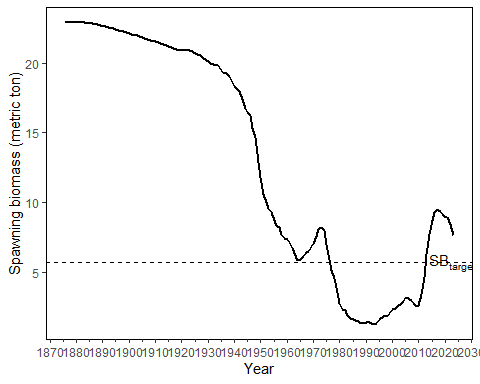
\includegraphics{SAR_USWC_Petrale_sole_skeleton_files/figure-docx/spawn_bio-1.png}

}

\caption{This is a great caption explaining a trend of spawning biomass
of Petrale sole in test in-line code 0.3 .}

\end{figure}%

\newpage{}

\section{Appendices}\label{appendices}



\end{document}
